\documentclass[12pt,aspectratio=169]{beamer}
\usetheme[version=2019]{iiasa}

\usepackage{ifthen}
\ifthenelse{\equal{\detokenize{notes}}{\jobname}}{%
\setbeameroption{show only notes}%
}{
%
}

\usepackage[
  maxnames = 1,
  style = authoryear,
  giveninits,
  terseinits,
  maxcitenames = 3,
  ]{biblatex}
\addbibresource{all.bib}
% Small font in bibliography
\renewcommand*\bibfont{\small}
\addbibresource{all.bib}

\usepackage{minted}
\usepackage{pdfpages}

\usepackage{tikz}
\usetikzlibrary{calc}

% https://tex.stackexchange.com/a/446296/94986
\newcommand{\side}[1]{
(0.0,#1*0.00) .. controls (0.0,#1* 0.00) and (0.4,#1*-0.04) ..
(0.4,#1*0.04) .. controls (0.4,#1* 0.11) and (0.2,#1* 0.26) ..
(0.5,#1*0.26) .. controls (0.8,#1* 0.26) and (0.6,#1* 0.11) ..
(0.6,#1*0.04) .. controls (0.6,#1*-0.04) and (1.0,#1* 0.00) ..
(1.0,#1*0.00)
}

\newcommand{\piece}[2][black]{
\begin{scope}[scale=2, shift={($(#2) - (0.25,0.48)$)}]
  \path [draw = #1, ultra thick, line cap = round]
  \side{1}  % Bottom; -1 is out, 1 is in
  [rotate around={90:(0.5,0.5)}] \side{1}    % Right
  [rotate around={180:(0.5,0.5)}] \side{-1}  % Left
  [rotate around={270:(0.5,0.5)}] \side{-1};  % Top
\end{scope}
}



\title{Effective strategies for multi-sectoral research using large-scale models}
\institute{Energy, Climate, and Environment (ECE) Program \\
  International Institute for Applied Systems Analysis (IIASA)}

\date{\texorpdfstring{ISSST 2021 / §ESST6 Integrated assessment and energy system modeling\\
  Wednesday, 23 June 2021 \hfill \href{https://paul.kishimoto.name/2021/06/issst}{paul.kishimoto.name/2021/06/issst}\ }%
  {2021-06-23}}

\author{\texorpdfstring{Dr. Paul Natsuo Kishimoto \scriptsize\newline
  \href{mailto:paul.kishimoto@iiasa.ac.at}%
       {\ttfamily <paul.kishimoto@iiasa.ac.at>}}%
  {Dr. Paul Natsuo Kishimoto <paul.kishimoto@iiasa.ac.at>}}

\begin{document}

\maketitle

\note{
Good day everyone, and thank you for joining for this talk on “effective strategies for multi-sectoral research using large-scale models”.

My name is Paul Kishimoto, and I am a research scholar in the ECE program at the International Institute for Applied Systems Analysis.

(15")}

\begin{frame}
\frametitle{Outline}

\tableofcontents

\end{frame}

\note{
This is a bit of an odd talk, because I'm going to jump from a high-level, conceptual, or meta perspective on model-based research, straight down to quotidian activities that we don't usually talk about when we present results.

In fact I'm not going to promote any particular study, but instead discuss \emph{how} we do research with models, and suggest some ways to improve that.

My hope, by the time I finish, is that you will also see the importance of these perspectives, and try applying them in your own work.

(50")}

\section{Motivation and concepts}
\begin{frame}
\frametitle{Motivation}

\begin{itemize}
  \item Pursuit of climate change mitigation and other SDGs entails \structure{changes in systems}—complex, large, interconnected, open, sociotechnical.%
  \footcite[or “CLIOS”, per][]{mostashari-sussman-2009}
  \item Quantitative computer models%
  \footnote{aka. analyses, workflows, tools, scripts.}
  are used to study these systems.
  \item Changes trouble the boundaries between ‘sectors’ of human/economic activity:
    \begin{itemize}
      \item Changes large enough that feedbacks from other sectors are non-negligible.
      \item New technologies establish new interactions, e.g. electric vehicle–grid interoperation.
    \end{itemize}
  \item We are motivated to \structure{connect sets (N≥2) of models} or \structure{increase complexity} to study changes in multiple subsystems at once.
\end{itemize}

\end{frame}

\note{
These sectoral boundaries have, of course, also become disciplinary boundaries.
}

\begin{frame}{Internal vs.\ external validity}
\framesubtitle{Concerns for scientific modeling \& scenario research}

\structure{Internal validity.} Research is free of errors:

\begin{itemize}
  \item Correctly implements theory w/o conceptual errors.
  \item Confounding variables addressed to identify relationships between independent and dependent variables.
  \item Alternative hypotheses can be rejected.
\end{itemize}

\bigskip
\structure{External validity.} Research is generalizable to other conditions:

\begin{itemize}
  \item Research can be replicated or reproduced in a different context.
  \item Research is robust to differences between the study context and other contexts to which conclusions are applied.
  \item Research is robust to plausible alternatives to key assumptions.
\end{itemize}

\end{frame}


\subsection{Three perspectives on models}
\begin{frame}[allowframebreaks]{What is a model?}
\framesubtitle{Three perspectives and resulting insights}

A \structure{knowledge object} that embodies or represents a theory or understanding of some real-world phenomenon.

\medskip
\begin{itemize}
  \item Theories often causal.
  \item Relationships expressed quantatively: equations connecting variables representing concepts measured in certain, systematic ways.
  \item In large-scale integrated assessment, systematized concepts often aggregate: GDP, country, sector.
\end{itemize}

\framebreak
A \structure{scientific instrument}\footcite{omalley-2019} that is used to perform experiments: “What would be the outcome (effect on quantity $Y$) if $X$ were changed from $x_1$ to $x_2$?”

\medskip
\begin{itemize}
  \item Another instrument: the Large Hadron Collider (LHC).
    \begin{itemize}
      \item EUR 7.5 billion budget; labour from many specialized roles.
      \item Components for preparing the experiment, running it, measuring outcomes are carefully designed, constructed, tested.
    \end{itemize}
  \item Instruments require meticulous attention to detail.
  \item Description of methods includes description of instruments, so the experiment can be reproduced.
\end{itemize}

\framebreak
A \structure{software project} in which people in organizations create code that is run on computer systems.

\medskip
\begin{itemize}
  \item All software has bugs; all organizations have politics.
  \item Software is constantly evolving and never complete.
  \item Tendency to overinvest time in new code vis-à-vis quality \& docs.
  \item “Technical debt”: code grows stale over time.
\end{itemize}

\med
\structure{\bfseries But!} good software development practices exist, and are widely used to ensure that software meets needs.

\end{frame}


\subsection{Validity, reproducibility, interoperability, reuse}
\begin{frame}{Validity and reproducibility}

Since the model is not the real world, implications drawn from modeling results must be externally valid.
Specific threats, as forms of uncertainty:

\begin{description}
  \item [Structural] Is the theory a correct description of the phenomena?

    → Response: alternate model formulations.

  \item [Measurement] uncertainty of input data and parameters.

    → Sensitivity analyses, large ($>10^3$) ensembles of model runs.

  \item [Epistemic] uncertainty in conditions (e.g. future policy) that are unknowable, or whereof uncertainty cannot be quantified.

    → Alternate scenarios.
\end{description}

All require a \structure{quality} instrument that can be \structure{reused in an easy, automated manner}, giving the \structure{same results every time}—a \structure{\bfseries reproducible} model.
\end{frame}

{
  \setbeamercolor{background canvas}{bg=}
  \setbeamertemplate{background}[default]
  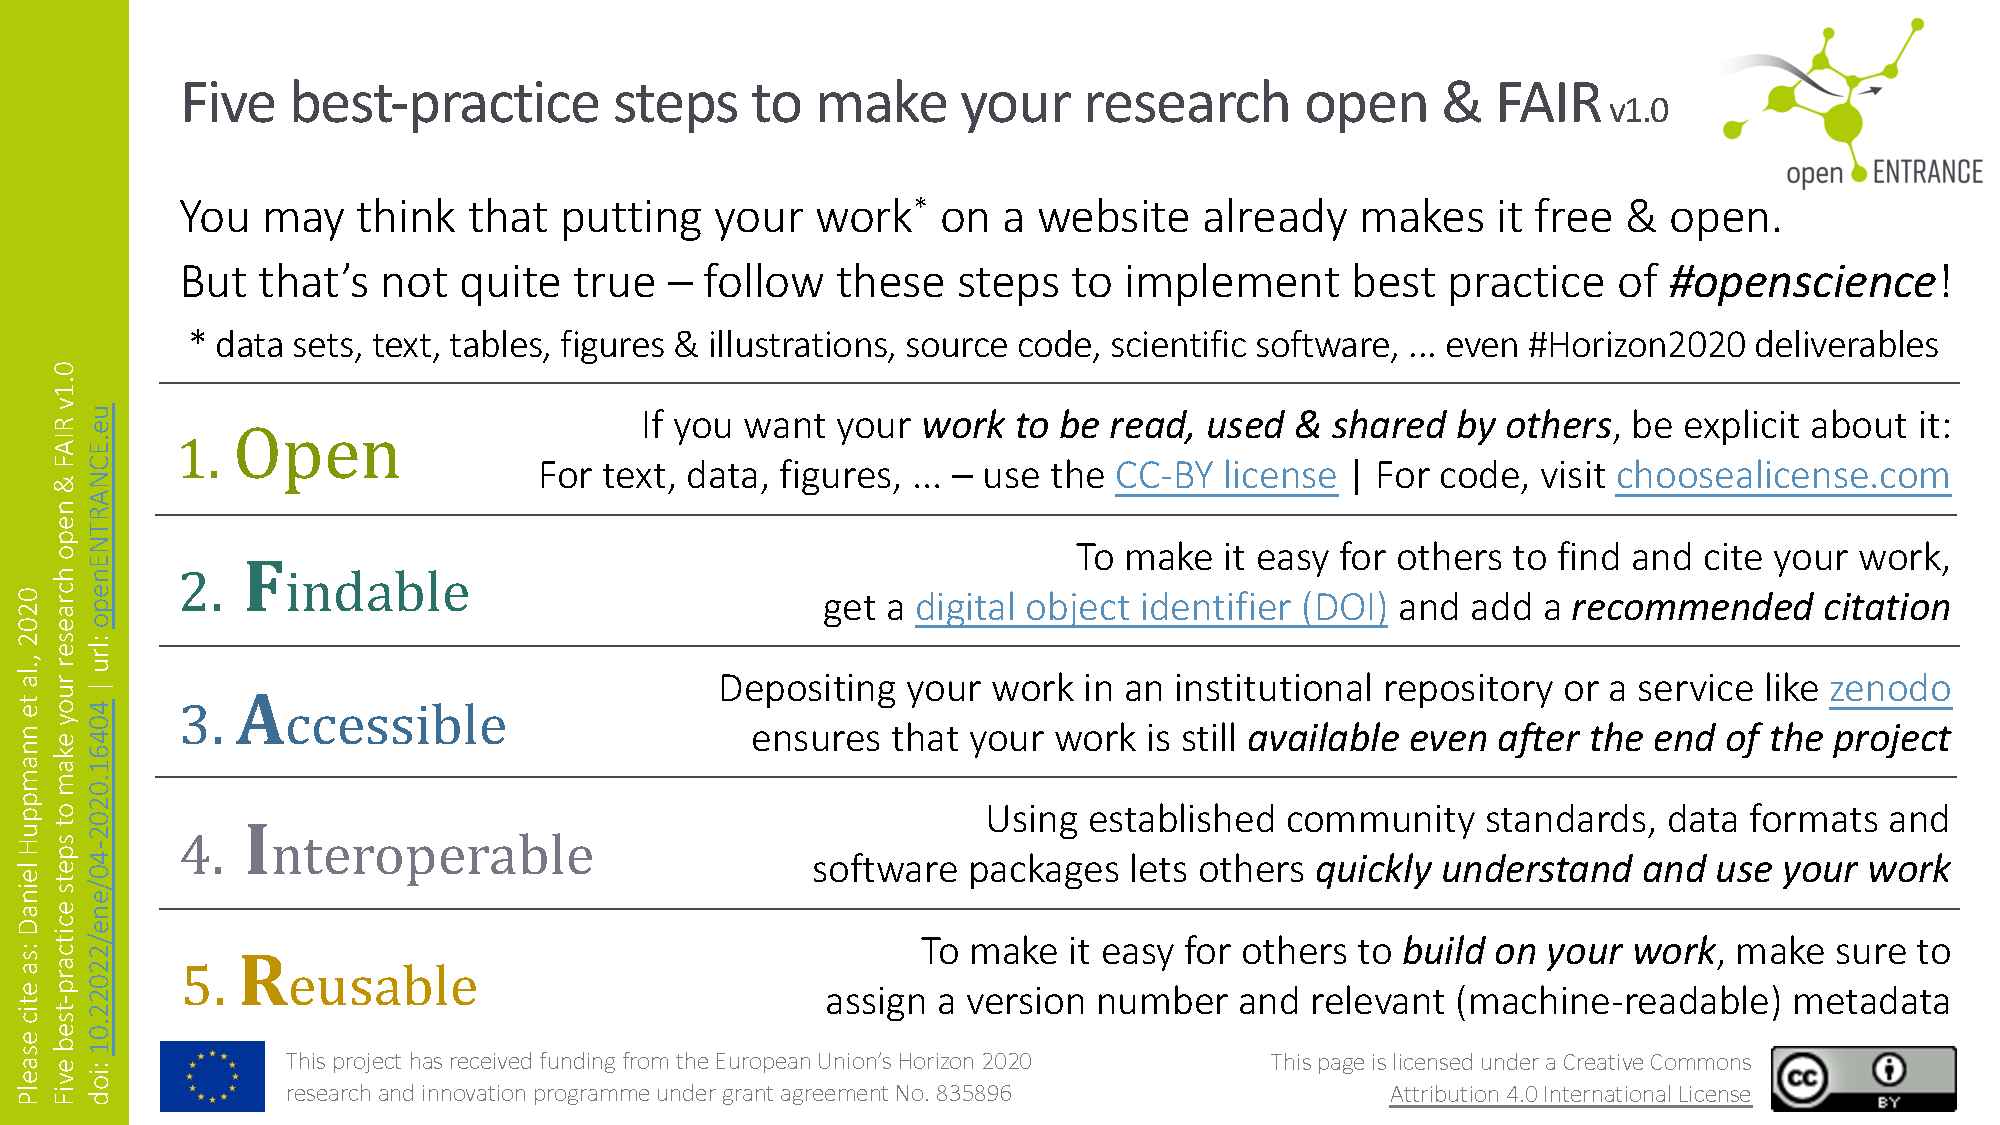
\includepdf{huppmann-2020.pdf}
}

\begin{frame}
\frametitle{“… Interoperable \& Reusable”}

Are these true \emph{in principle} or \emph{in practice}?
\begin{itemize}
  \item Easy to claim that others \structure{could, in principle}, re-use elements of a model-based research workflow.
  \item Much harder: make this an \structure{actual practice}, i.e. feasible with resources ≥1 others have.
\end{itemize}

\medskip
Even achievable reproduction is not true reusability.
\begin{itemize}
  \item \structure{Equity \& inclusion} require that analytical tools and capabilities be broadly distributed.
  \item Not adequate that researchers from LMICs join well-resourced incumbent modeling teams, if these remain central.
  \item Urgency of climate change \& SDGs requires we bring more hands to the work.
\end{itemize}

\end{frame}

\note{
The key question to ask is always: has someone actually managed to reuse this tool?
Has someone made it interoperate with another?

The goal of equity sets an even higher bar.
I won't go on about this; I'll only say: If someone can or does reuse my tools, but I always have to be involved in that to support them, and be compensated in some way for that work, then I centre myself and I limit the work that can be done to the number of people that I or my group can support.
}

\subsection{Costs, resources}
\begin{frame}
\frametitle{Costs \& resources}

We have finite resources (time etc.) with which to conduct research.
Work to create and use models should spend resources efficiently.

\smallskip
\structure{Search \& information}
\begin{itemize}
  \item How do I run the model? What does this line of code do?
  \item What about student S, who did … 2 years ago—where is that?
  \item What version of the model produced results for this 1 y/o manuscript?
\end{itemize}

\structure{Quality control \& enforcement}
\begin{itemize}
  \item When/why did our reference forecast shift in region $r$ \& sector $g$?
  \item Who broke the model so Policy Z no longer has a feasible solution?
\end{itemize}

\structure{Recovery/disruption}
\begin{itemize}
  \item If colleague C left tomorrow, could we continue our work?%
  \footnote{aka. the bus factor or truck number.}
\end{itemize}

\end{frame}


\begin{frame}
\frametitle{None of this is new}
\framesubtitle{or, standing on the shoulders of giants}

\begin{columns}[T]
\column{0.45\paperwidth}
Reproducibility crisis in quantitative social sciences, e.g. psychology.

\bigskip
Computing as fundamental to valid research: atmospheric \& climate sciences, engineering disciplines (cf. Barba et al.; see appendix), basic sciences.

\bigskip
Most practices from software industries; minor adjustments.

\column{0.5\paperwidth}
\centering
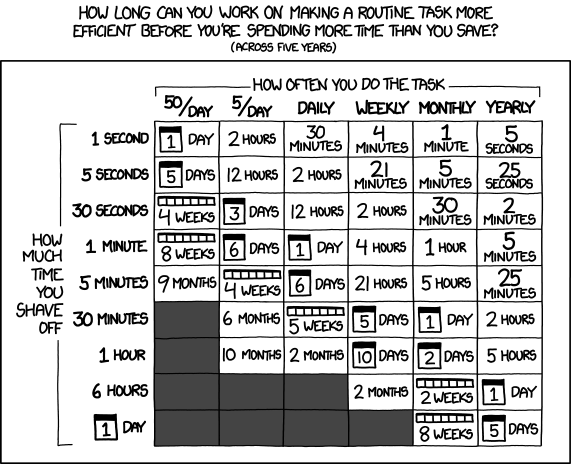
\includegraphics[width=\columnwidth]{xkcd_1205.png}
\url{https://xkcd.com/1205/}

\end{columns}

\end{frame}

\section{Practices for model-based research}
\begin{frame}
\frametitle{Examples from MESSAGE\emph{ix}-GLOBIOM}

\begin{description}
  \item [MESSAGE\emph{ix}] Generalized formulation for an energy-economic/integrated assessment LP model. \\
  {\bfseries \url{https://docs.messageix.org} \\ \url{https://github.com/iiasa/message_ix}}
  \item [MESSAGE\emph{ix}-GLOBIOM] A family of global and single-country models and variants built in this framework.
  \item [\ttfamily ixmp] Data storage backend \& solver interface.
  \item […] related tools for data, etc.
\end{description}

\bigskip
Caveats:
\begin{itemize}
  \item We aren't perfectly ‘OFAIR’ yet. This talk = mix of status \& goals.
  \item We celebrate continual improvement \& efforts of others to improve.
\end{itemize}

\end{frame}

\begin{frame}
\frametitle{Strategy and practice for modeling}

Start with organizational culture:
\begin{itemize}
  \item Discuss and identify in your team where resources are spent.
  \item Look for possible improvements in practice.
  \item Agree that there is a positive return on investment.
\end{itemize}

\bigskip
A collection of interlinked and mutually-reinforcing practices.
\begin{itemize}
  \item “A truly remarkable variety of practices, but these slides are too few to contain them.”
  \item Can be adopted separately, incrementally.
  \item Also corresponding skills → support skills development in your team.
\end{itemize}

\end{frame}

\begin{frame}[plain]
\tableofcontents[currentsection]
\end{frame}

\subsection{Use version control; write documentation}
\begin{frame}
\frametitle{The basics: version control, docs}

Use version control.
\begin{itemize}
  \item \url{https://github.com/iiasa/message_ix}
  \item Use fewer, larger, better-organized repositories.
  \item Learn and use the GitHub workflow.
\end{itemize}

\bigskip
Write (and read) documentation.
\begin{itemize}
  \item The \#1 audience for this is \emph{you}, or your closest collaborators.
  \item Rubber duck \& pair program: explain to a duck what the code does.
  \item Use services like Read The Docs: automate build \& publish steps for every change to the code.%
  \footnote{\href{https://readthedocs.com/projects/iiasa-energy-program-message-ix/}{Recent builds of the MESSAGE\emph{ix} docs}.}
\end{itemize}

\end{frame}

\subsection{Write modular code for reuse}
\begin{frame}
\frametitle{Write modular code for reuse}

Common to have a variety of tasks in one (very long) “script” (or a few):
\begin{itemize}
  \item Input data processing, assumptions, bits of methods adopted from literature, core methods/workflow, post-processing/plotting, output, logging…
\end{itemize}

\bigskip
Instead, and \structure{from the start}:
\begin{itemize}
  \item Separate concerns: 1 task per code object; files group related tasks.
  \item DRY: don't repeat yourself. Write \& reuse functions and classes → fewer occasions for error.
  \item Smaller, atomic functions \& classes are easier to document, understand, and validate.%
    \footnote{Often can be discarded in favour of high-quality, performant ones\\ \hspace{25mm} from popular libraries; read the docs!}
  \item New data, methods, etc. can be easily swapped-in.
\end{itemize}

\end{frame}

\subsection{Write tests (=internal validity)}
\begin{frame}[fragile]
\frametitle{Write tests for internal validity}

Software tests = code that runs other code, giving a “pass” or “fail” result.

\smallskip
\begin{minted}{python}
def test_stock(dummy_data):
    observed = compute_vehicle_stock(dummy_data)
    expected = 42.1
    assert observed == expected
\end{minted}

\smallskip
Code that implements core theory/methods can be tested for a variety of inputs $\equiv$ checks of internal validity.

\bigskip
MESSAGE\emph{ix}: 100s of tests from basic (data I/O) to complex functionality (LP constraint relaxation; dynamic penetration of new technologies…)

→ \href{https://github.com/iiasa/message_ix/tree/main/message_ix/tests}{github.com/iiasa/message\_ix/tree/main/message\_ix/tests}

\end{frame}

\subsection{Automate, towards “continuous reproduction”}
\begin{frame}
\frametitle{Automate}
\framesubtitle{towards “continuous reproduction”}

\structure{Continuous integration} (CI) services:
\begin{itemize}
  \item Watch a code repository, e.g. on GitHub, for changes.
  \item Automatically grab new versions.
  \item Perform certain actions, e.g. run a suite of tests.
\end{itemize}

\medskip
Tests cover \emph{all core methods} in a model → CI reduces work to guard against \structure{invalidity} when improving models (‘reggressions’).

\medskip
Code includes \emph{all steps} in a model-based analysis → CI system can \structure{continuous confirm reproducibility}.

Example: A \href{https://github.com/iiasa/message_ix/blob/main/tutorial/westeros/westeros_baseline.ipynb}{tutorial notebook} from MESSAGE\emph{ix}.
\begin{itemize}
  \item Constructs and solves a simple energy system model.
  \item Full-scale models currently private (proprietary data).
\end{itemize}

\end{frame}


\section{Practices for multi-sector research}

\begin{frame}[plain]
\tableofcontents[currentsection]
\end{frame}

\subsection{Separate model-building components}
\begin{frame}
\frametitle{Separate model-building components}

Separate code that prepares a “base” model from code that adds/alters detail \& resolution related to a particular phenomenon or sector.

\bigskip
\begin{tikzpicture}
  \node (m-g) {Global};
  \piece[IIASAblue]{m-g}

  \only<1-2>{
  \node [anchor=west] at ($(m-g.east) + (1, 0)$)
    {$\leftarrow$ instance of the global MESSAGE\emph{ix}-GLOBIOM model};
  }

  \only<1-3>{\coordinate (m-t-pos) at ($(m-g.center) + (5, 0)$);}
  \only<4>{\coordinate (m-t-pos) at ($(m-g.center) + (2, 0)$);}

  \only<3->{
  \node (m-t) at (m-t-pos) {Transport};
  \piece[IIASAgreen]{m-t}
  }

  \only<4>{
  \node [anchor=west] at ($(m-t.east) + (1, 0)$)
    {$\leftarrow$ global model + added transport-sector resolution};
  }
\end{tikzpicture}

\end{frame}

\begin{frame}
\frametitle{Separate model-building components}

\begin{columns}
\column{0.3\paperwidth}
\begin{tikzpicture}
  \node (m-g) {Global};
  \piece[IIASAblue]{m-g}

  \coordinate (m-t-pos) at ($(m-g.center) + (2, 0)$);

  \node (m-t) at (m-t-pos) {Transport};
  \piece[IIASAgreen]{m-t}
\end{tikzpicture}

\column{0.6\paperwidth}
Each of these pieces is under continual development by separate teams of researchers.
This \emph{could} entail frequent and laborious adjustments.

\bigskip
\pause Modularity + testing ensure that the “shape of the piece” (structure and data of the model prepared by some code) is stable.

\smallskip
\pause → base “Global” model presents the same shape.

\pause → code that configures the “Transport” variant works on anything that has this shape.
\end{columns}
\end{frame}

\begin{frame}
\frametitle{Separate model-building components}

Pieces can “be plugged in” to any base or enhanced model, so long as it presents the right shape $\equiv$ valid models can be composed with details required for particular studies.

\medskip
\centering
\begin{tikzpicture}[every node/.style = {text depth = 0.3ex}]
  \node (m-g) {Global};
  \piece[IIASAblue]{m-g}

  \only<1>{\coordinate (mt-pos) at ($(m-g.center) + (4, 1.5)$);}
  \only<2>{\coordinate (mt-pos) at ($(m-g.center) + (2, 0)$);}
  \only<3>{\coordinate (mt-pos) at ($(m-g.center) + (6, 0)$);}

  \node (mt) at (mt-pos) {Transport};
  \piece[IIASAgreen]{mt}

  \only<1>{\coordinate (bldg-pos) at ($(m-g.center) + (4, -1.5)$);}
  \only<2>{\coordinate (bldg-pos) at ($(m-g.center) + (4, 0)$);}
  \only<3>{\coordinate (bldg-pos) at ($(m-g.center) + (8, 0)$);}

  \node (bldg) at (bldg-pos) {Buildings};
  \piece[IIASApurple]{bldg}

  \only<1>{\coordinate (IL-pos) at ($(m-g.center) + (8, 1.5)$);}
  \only<2>{\coordinate (IL-pos) at ($(m-g.center) + (8, 0)$);}
  \only<3>{\coordinate (IL-pos) at ($(m-g.center) + (2, 0)$);}

  \node (IL) at (IL-pos) {Materials};
  \piece[IIASAred]{IL}

  \only<1>{\coordinate (sa-pos) at ($(m-g.center) + (8, -1.5)$);}
  \only<2>{\coordinate (sa-pos) at ($(m-g.center) + (6, 0)$);}
  \only<3>{\coordinate (sa-pos) at ($(m-g.center) + (4, 0)$);}

  \node (sa) at (sa-pos) {Water};
  \piece[IIASAteal]{sa}
\end{tikzpicture}

\medskip
\uncover<3>{
Our implementation: in the \href{https://docs.messageix.org/projects/models2/en/latest/api/model-build.html}{\ttfamily message-ix-models} package.
}

\end{frame}

\subsection{Be precise about metrology; use “data interfaces”}
\begin{frame}[allowframebreaks]
\frametitle{Use precise metrology}

Specify data flows separately from methods:
\smallskip

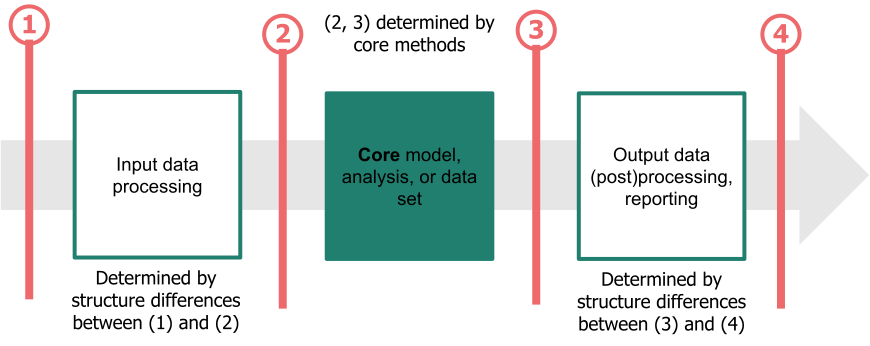
\includegraphics[width=\columnwidth]{data-stages}

These form another kind of \structure{interface} and help towards \structure{interoperability}.

\framebreak

At each interface (1) through (4) be precise about:
\begin{itemize}
  \item Background vs. systematized concepts vs. specific measures.\footcite{adcock-collier-2001}
  \item Dimensions, and the specific codes%
    \footnote{e.g. \texttt{Canada} vs. \texttt{CAN} vs. \texttt{CA}; \href{https://paul.kishimoto.name/2021/01/handling-country-codes/}{read more}.}
    used along each.
  \item Units of measurement. (Check with \href{https://pint.readthedocs.io}{Pint} or similar.)
\end{itemize}

\medskip
Treat all assumptions as input data → none in code.

\medskip
Don't invent new data formats:
\begin{itemize}
  \item Reuse existing formats and protocols for exchange

    e.g. SDMX (\href{https://sdmx.org}{1}, \href{https://sdmx1.readthedocs.io/en/latest}{2}), \href{https://www.unidata.ucar.edu/software/netcdf/}{NetCDF}, \href{https://zarr.readthedocs.io/en/stable/}{Zarr}, etc.
  \item Reuse existing (or shared) codes, categorizations, and labels

    e.g. \href{https://en.wikipedia.org/wiki/List_of_ISO_3166_country_codes}{ISO 3166-1}; \href{https://registry.sdmx.org/items/codelist.html}{SDMX global registry}.
\end{itemize}

\end{frame}


\section{Conclusions}
\begin{frame}[allowframebreaks]
\frametitle{Conclusion: back to costs}
Not mentioned earlier: cost of disobeying incentives.

\bigskip
Some incentives that can affect us as model-builders and -users:
\begin{itemize}
  \item Publish; only work that can be claimed ‘novel’, and only when final.
  \item Signal compliance with disciplinary norms with minimal effort.
  \item Assist only collaborators / co-authors; neglect others.
  \item Don't budget for maintenance and support.
  \item Value ‘Impressive’ polish, GUIs, and ease of rudimentary use…

    …over ‘mundane’ validation and reducing I \& R costs.
\end{itemize}

\framebreak
In contrast, free software—thus also \structure{open science}—succeeds when:
\begin{itemize}
  \item Communities work together to build a smaller number of higher-quality projects that are public goods.
  \item Innovation is planned \& done out in the open.
  \item Support, documentation, and enabling others' contributions is first-class, valued work.
\end{itemize}

\bigskip
→ not the same activities, shared \emph{ex post}; but a dramatic change in norms.

\bigskip
\hfill {\Large \structure{Thank you!}}
\end{frame}

\appendix

\section{Appendix}

\begin{frame}[allowframebreaks]
\frametitle{References \& further reading}

\nocite{huppmann-2020}
\printbibliography[heading=none]

\begin{itemize}
  \small
  \item L. Barba group @ GWU SEAS: \href{http://lorenabarba.com/blog/barbagroup-reproducibility-syllabus/}{r13y syllabus} w/readings on research group website; \citetitle{barba-2017}.
  \item Other disciplines: \cite{irving-2016}, \cite{pauliuk-2019}.
  \item Max Planck Institute for Meteorology \href{http://mpimet.mpg.de/en/science/publications/good-scientific-practice.html}{``Good scientific practice''} policy, rules, forms.
  \item Christensen \& Miguel (2016), \href{http:/dx.doi.org/10.3386/w22989}{``Transparency, Reproducibility, and the Credibility of Economics Research''} forthcoming in \emph{JEL} — UC Berkeley Econ.
  \item Nick Barnes: \href{https://www.nature.com/news/2010/101013/full/467753a.html}{``Publish your computer code: it is good enough''} in \emph{Nature News} — Climate Code Foundation.
  \item \href{http://ropensci.github.io/reproducibility-guide/sections/references/}{45+ more peer-reviewed articles} and other resources.
\end{itemize}

\medskip
\structure{Colophon}

PDF and abstract: \href{http://paul.kishimoto.name/2021/06/issst}{paul.kishimoto.name/2021/06/issst}

LaTeX source, copyright, \& license: \href{https://github.com/khaeru/doc/}{github.com/khaeru/doc}
\medskip

\end{frame}

\end{document}
